\subsection{Seed Synthesizer}

$\tool$ synthesizes seed programs using two synthesizers.

\subsubsection{Non-Recursive Synthesizer}
The first synthesizer aims to cover as many syntax cases as possible
in two steps: 1) to find the shortest string for each non-terminal
and 2) to synthesize JavaScript programs using the shortest strings.
For presentation brevity, we explain simple cases like terminals and non-terminals,
but the implementation supports the extended grammar of
ECMAScript such as parametric non-terminals, conditional alternatives,
and special terminal symbols.

\begin{algorithm}[t]
  \caption{Worklist-based Shortest String}
  \label{alg:short-string}
  \DontPrintSemicolon
  \SetKwProg{Fn}{Function}{:}{}
  \SetKwFunction{shortestStrings}{shortestStrings}
  \SetKwFunction{update}{update}
  \SetKwFunction{propagate}{propagate}
  \KwIn{$\ruleset$ - syntax reduction rules}
  \KwOut{$M$ - map from non-terminals to shortest strings derivable
    from them}
  \Fn{\shortestStrings{$\ruleset$}} {
    $M = \varnothing, \worklist = \text{a queue that contains}\ \ruleset$\;
    \While{$\worklist \neq \varnothing$} {
      $\text{pop}\ (A, \alpha) \gets \worklist$\;
      \lIf{$\update(A, \alpha)$} {
        $\propagate(\worklist, \ruleset, A)$}
    }
  }
  \Fn{\update{$A, \alpha$}} {
    $str = \text{an empty string}$\;
    \ForAll{$s \in \alpha$} {
      \lIf{$s\ \text{is a terminal}\ t$} {
        $str = str + t$
      }
      \ElseIf{$s\ \text{is a non-terminal}\ A' \wedge A' \in M$} {
        $str = str + M[A']$
      }
      \lElse {
        \Return false
      }
    }
    \lIf{$\exists M[A] \wedge \norm{str} \geq \norm{M[A]}$} {
      \Return false
    }
    $M[A] = str$\;
    \Return true\;
  }
  \Fn{\propagate{$\worklist, \ruleset, A$}} {
    \ForAll{$(A', \alpha') \in \ruleset$} {
      \lIf{$A \in \alpha'$} {
        $\text{push}\ (A', \alpha') \rightarrow \worklist$
      }
    }
  }
\end{algorithm}

The \mytextsf{shortestStrings} function in Algorithm~\ref{alg:short-string} shows the first step.
We modified McKenize's algorithm~\cite{cfg-gen} that finds random
strings to find the shorted string.  It takes syntax reduction rules
$\ruleset$, a set of pairs of non-terminals and alternatives, and
returns a map $M$ from non-terminals to shortest strings derivable from them.
It utilizes a worklist $W$, a queue structure that includes syntax reduction rules
affected by updated non-terminals.
The function initializes the worklist $W$ with all the syntax reduction rules $\ruleset$.
Then, for a syntax reduction rule $(A, \alpha)$, it updates the
map $M$ via the \mytextsf{update} function, and propagates updated
information via the \mytextsf{propagate} function.
The \mytextsf{update} function checks whether a given alternative $\alpha$ of
a non-terminal $A$ can derive a string shorter than the current
shortest one using the current map $M$.
If possible, it stores the mapping from the non-terminal $A$ to the
newly found shortest string in $M$ and invokes \mytextsf{propagate}.
The \mytextsf{propagate} function finds all the syntax reduction rules
whose alternatives contain the updated non-terminal $A$ 
and inserts them into $W$.  The \mytextsf{shortestStrings} function
repeats this process until the worklist $W$ becomes empty.

\begin{algorithm}[t]
  \caption{Non-Recursive Synthesize}
  \label{alg:non-rec-synthesize}
  \DontPrintSemicolon
  \SetKwProg{Fn}{Function}{:}{}
  \SetKwFunction{nonRecSynthesize}{nonRecSynthesize}
  \SetKwFunction{getProd}{getProd}
  \SetKwFunction{getAlt}{getAlt}
  \KwIn{$\ruleset$ - syntax reduction rules, $S$ - start symbol}
  \KwOut{$D$ - set of strings derivable from $S$}
  \SetKwBlock{Begin}{function}{end function}
  \Fn{\nonRecSynthesize{$\ruleset, S$}} {
    $V = \varnothing, M = \shortestStrings(\ruleset)$\;
    \Return $\getProd(M, V, \ruleset, S)$\;
  }
  \Fn{\getProd{$M, V, \ruleset, A$}} {
    \lIf{$A \in V$} {
      \Return $\{ M[A] \}$
    }
    $D = \varnothing, V = V \cup \{ A \}$\;
    \ForAll{$(A', \alpha) \in \ruleset\ \text{s.t.}\ A' = A$} {
      $D = D \cup \getAlt(M, V, \ruleset, A, \alpha)$\;
    }
    \Return $D$\;
  }
  \Fn{\getAlt{$M, V, \ruleset, A, \alpha$}} {
    $L = \text{an empty list}$\;
    \ForAll{$s \in \alpha$} {
      \If{$s\ \text{is a terminal}\ t$} {
        $\text{append}\ (\{ t \}, t)\ \text{to}\ L$\;
      }
      \ElseIf{$s\ \text{is a non-terminal}\ A'$} {
        $\text{append}\ (\getProd(M, V, \ruleset, A'), M[A])\ \text{to}\ L$}
    }
    $D =$ point-wise concatenation of first elements of pairs in $L$ using
    second elements as default ones.\;
    \Return $D$\;
  }
\end{algorithm}

Using shortest strings derivable from non-terminals, 
the \mytextsf{nonRecSynthesize} function in Algorithm~\ref{alg:non-rec-synthesize}
synthesize programs.  It takes syntax reduction rules $\ruleset$ and a start symbol $S$.
For the first visit with a non-terminal $A$, the \mytextsf{getProd} function returns
strings generated by \mytextsf{getAlt} with alternatives of the non-terminal $A$.
For an already visited non-terminal $A$, it returns the single shortest string $M[A]$.
The \mytextsf{getAlt} function takes a non-terminal $A$ with an alternative
$\alpha$ and returns a set of strings derivable from $\alpha$ via
point-wise concatenation of strings derived by symbols of $\alpha$.
When the numbers of strings derived by symbols are different,
it uses the shortest strings derived by symbols as default strings.

\begin{figure}[t]
  \centering
  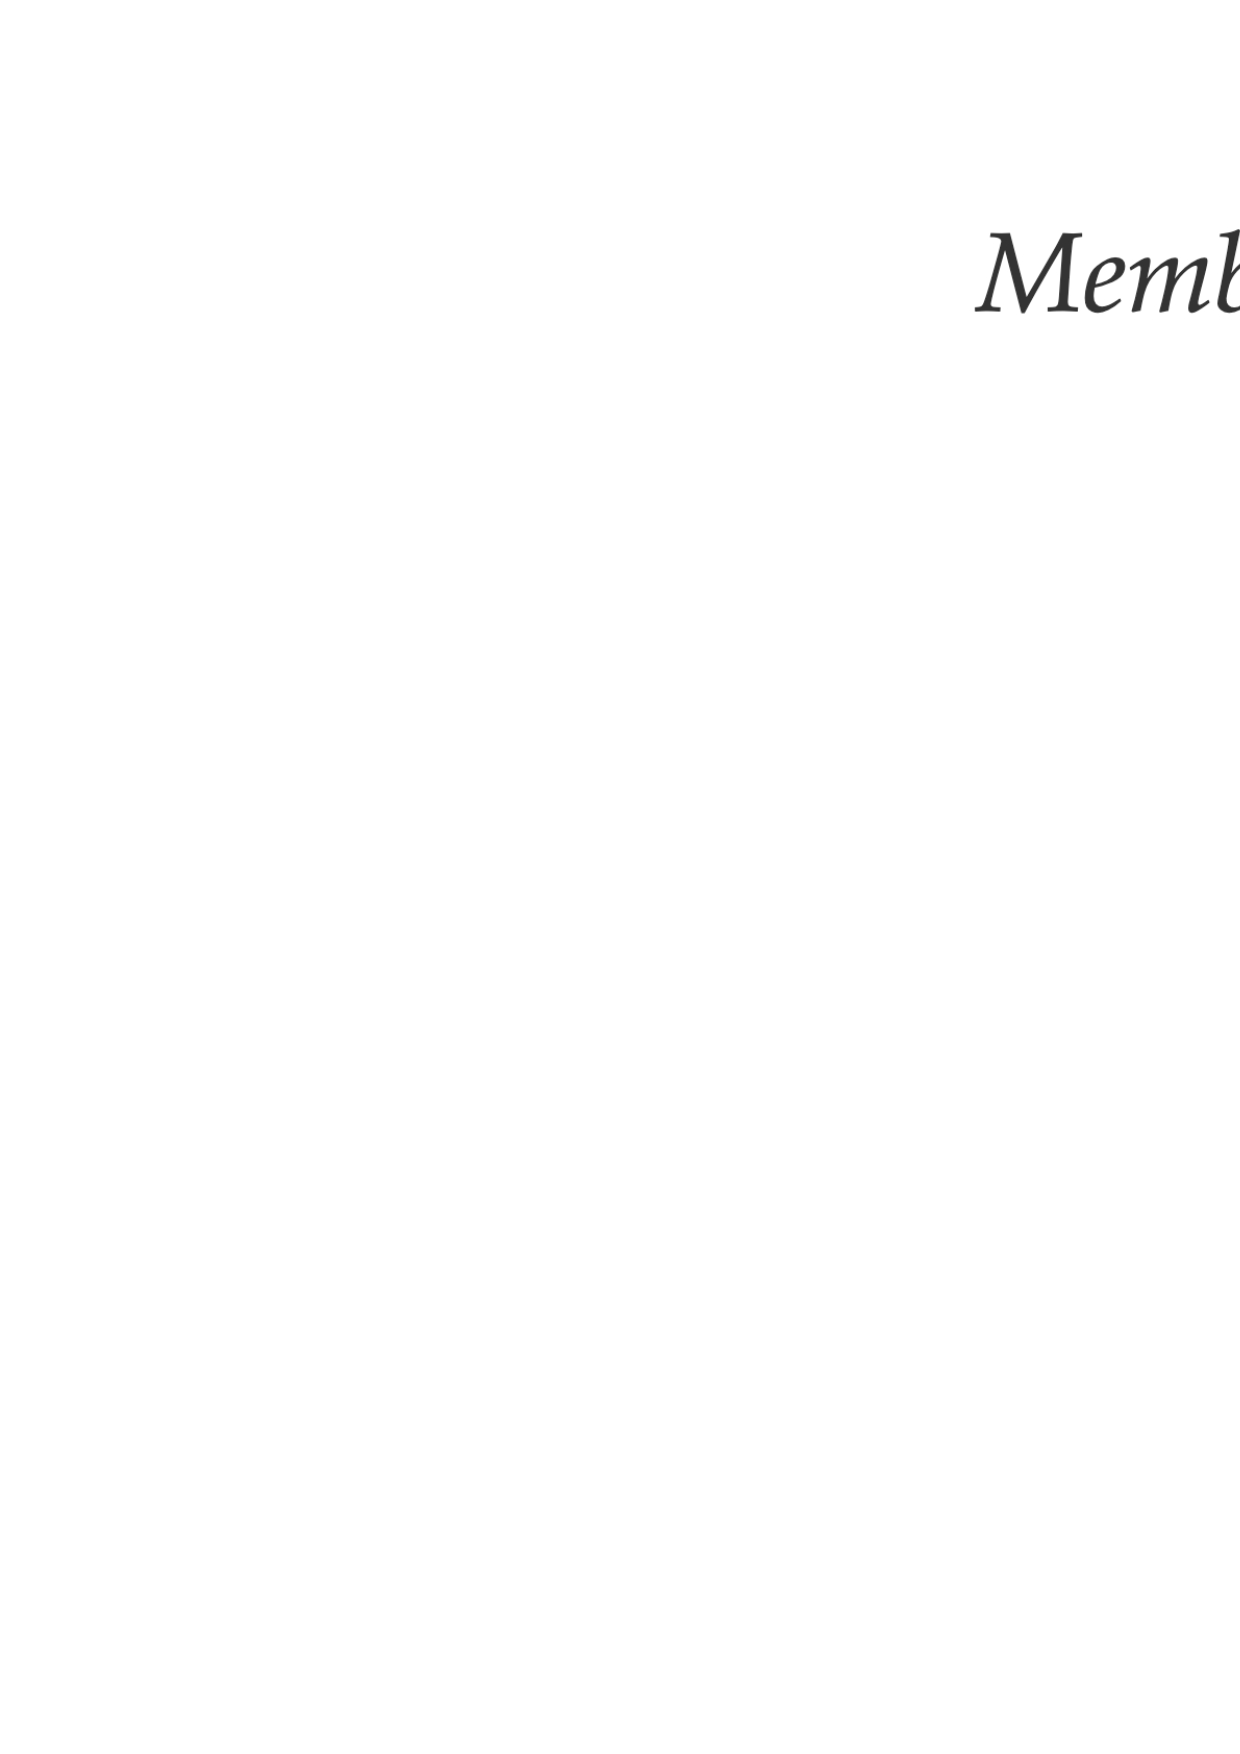
\includegraphics[width=0.31\textwidth]{img/syntax-member.pdf}
  \caption{The \textit{MemberExpression} production in ES11}
  \label{fig:prod-example}
  \vspace*{-1em}
\end{figure}

For example, Figure~\ref{fig:prod-example} shows a simplified
\textit{MemberExpression} production in ES11.  For the first step, we find
the shortest string for each non-terminal: \code{()} for \textit{Arguments} and
\code{x} for the other non-terminals.  Note that we use pre-defined shortest
strings for identifiers and literals such as \code{x} for identifiers and
\code{0} for numerical literals.  In the next step, we synthesize strings
derivable from \textit{MemberExpression}.  The first alternative is a
single non-terminal \textit{PrimaryExpression}, which is never visited.
Thus, it generates all cases of \textit{PrimaryExpression}.  The fourth
alternative consists of one terminal \code{new} and two non-terminals
\textit{MemberExpression} and \textit{Arguments}.  Because \textit{MemberExpression}
is already visited, it generates a single shortest string \code{x}.
For the first visit of \textit{Arguments}, it generates all cases:
\code{()}, \code{(x)}, \code{(...x)}, and \code{(x,)}.
Note that the numbers of strings generated for symbols are different.
In such cases, we use the shortest strings for symbols like
\code{x} for \textit{MemberExpression} as follows:

\vspace*{-.5em}
\begin{figure}[H]
  \centering
  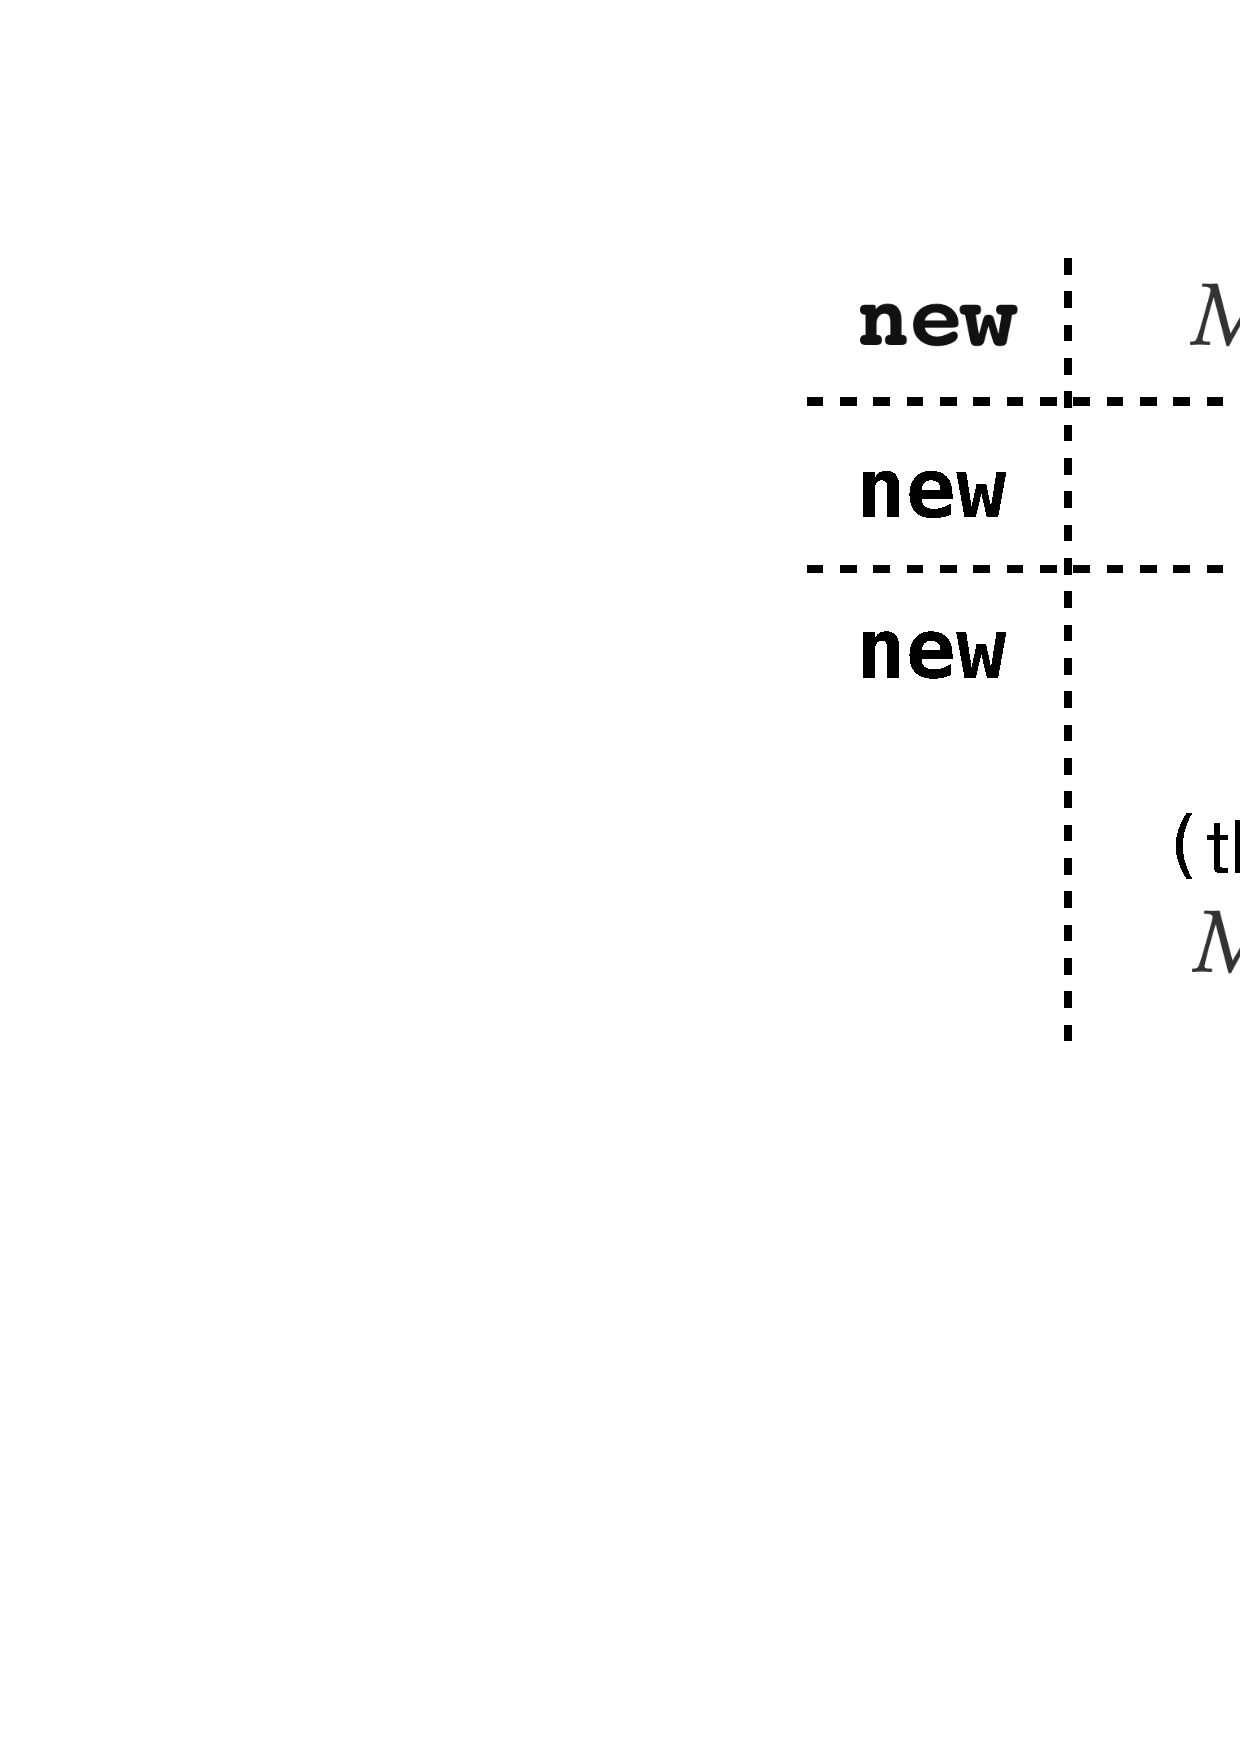
\includegraphics[width=0.46\textwidth]{img/member-example.pdf}
\end{figure}
\vspace*{-.5em}

\subsubsection{Built-in Function Synthesizer}

JavaScript supports diverse built-in functions for primitive values and built-in objects.
To synthesize JavaScript programs that invoke built-in functions,
we extract the information of each built-in function from the mechanized ECMAScript.
We utilize the \code{Function.prototype.call} function to invoke
built-in functions to easily handle the \code{this} object in \mytextsf{Program Mutator};
we use a corresponding object or \code{null} as the \code{this} object by default.
In addition, we synthesize function calls with optional and variable number of arguments
and built-in constructor calls with the \code{new} keyword.

Consider the following \code{Array.prototype.indexOf} function for
JavaScript array objects that have a parameter \textit{searchElement}
and an optional parameter \textit{fromIndex}:

\vspace*{-.5em}
\begin{figure}[H]
  \centering
  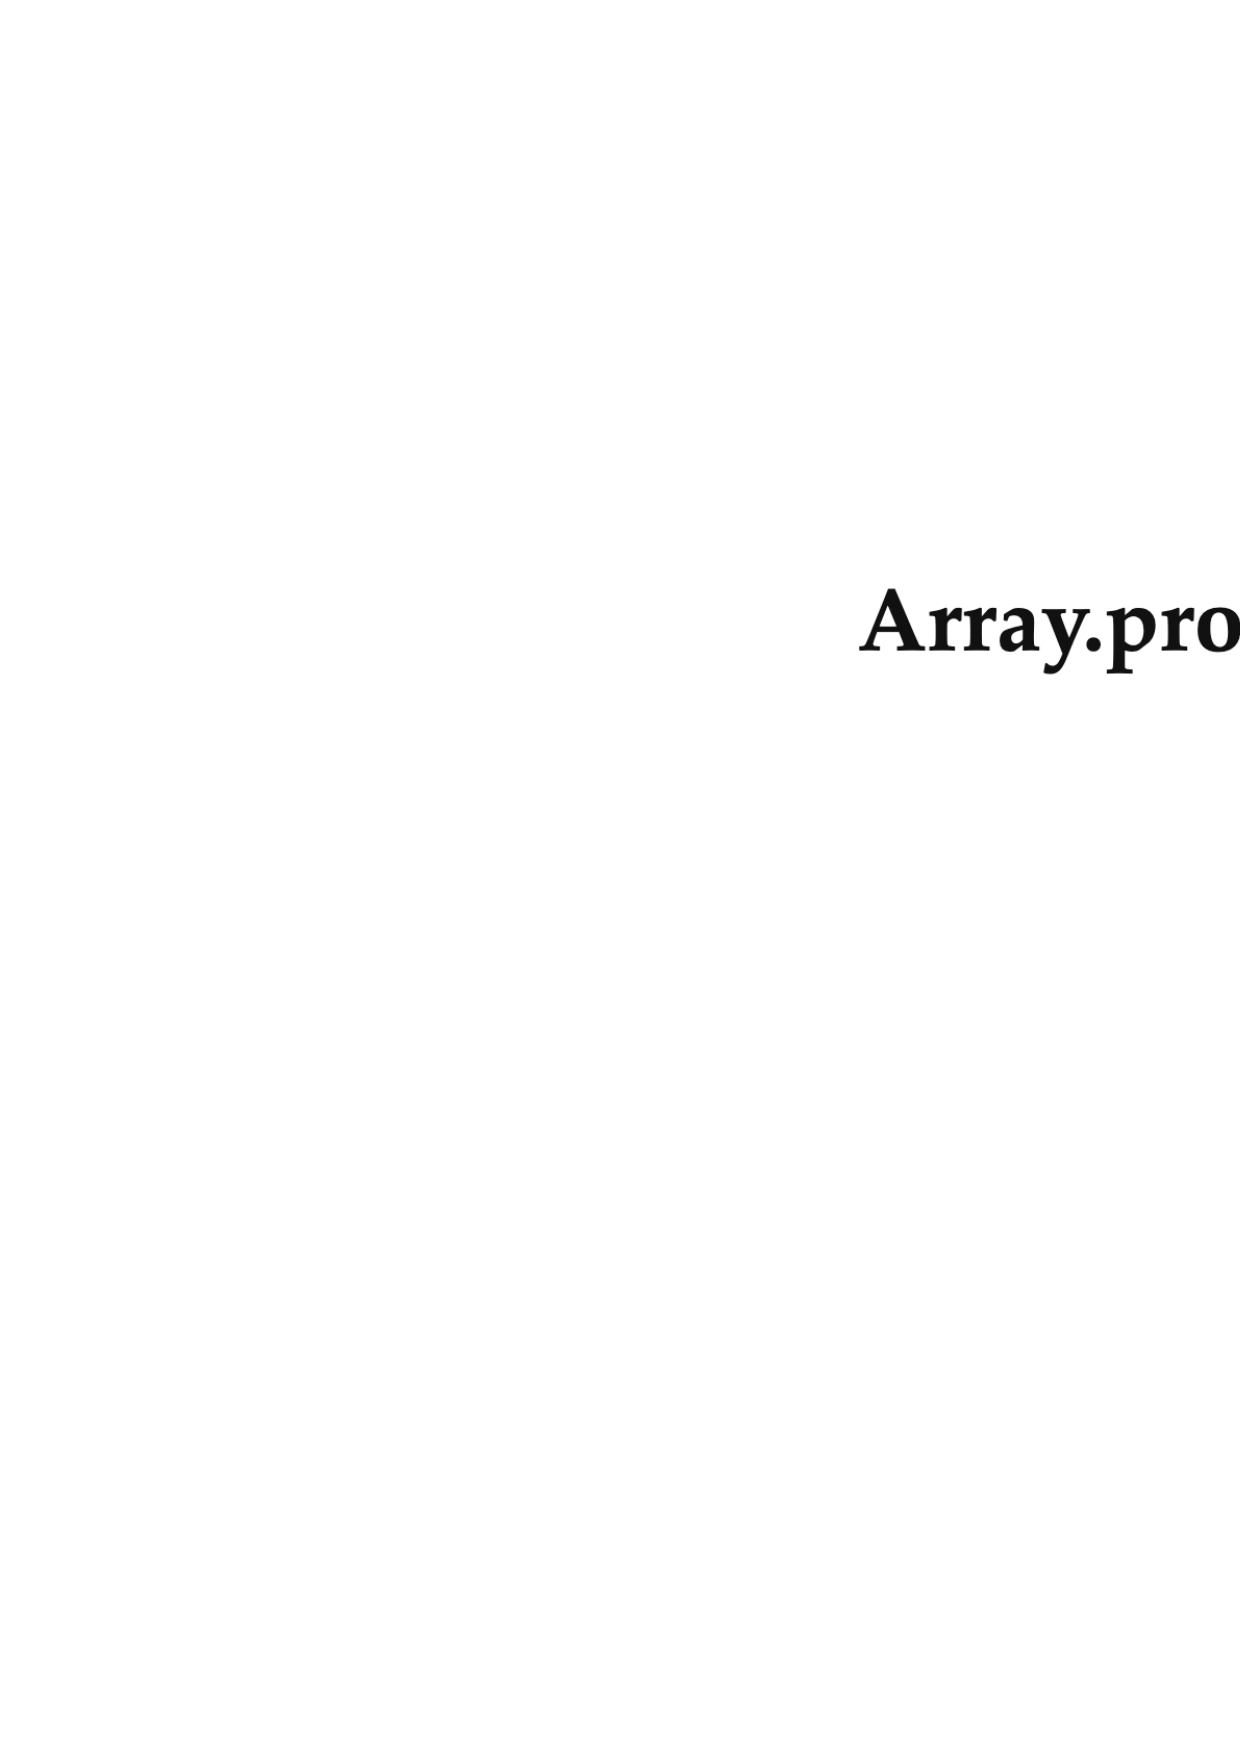
\includegraphics[width=0.4\textwidth]{img/array-indexof.pdf}
\end{figure}
\vspace*{-.5em}

\noindent
the synthesizer generates the following calls with an array object or \code{null} as the \code{this}
object as follows:
\begin{lstlisting}[style=myJSstyle]
  Array.prototype.indexOf.call(new Array(), 0);
  Array.prototype.indexOf.call(new Array(), 0, 0);
  Array.prototype.indexOf.call(null, 0);
  Array.prototype.indexOf.call(null, 0, 0);
\end{lstlisting}
Moreover, \code{Array} is a built-in function and
a built-in constructor with a variable number of arguments.
Thus, we synthesize the following six programs for \code{Array}:
\begin{lstlisting}[style=myJSstyle]
    Array();      Array(0);      Array(0, 0);
    new Array();  new Array(0);  new Array(0, 0);
\end{lstlisting}
